\documentclass[aspectratio=169,9pt]{beamer}
\mode<presentation> 
\usepackage[utf8]{inputenc}
\usepackage{sansmathaccent} %Für equations
\usepackage{amsmath}
\usepackage{tikz}
\usepackage{multicol}
\usepackage{cancel}
\usepackage{relsize}
\usepackage{graphicx}
\usepackage[table]{xcolor}
\usepackage{fontawesome5}
\usepackage{enumitem}
\usepackage[labelfont={bf},font={color=black!40,footnotesize},tablename={Tabelle},figurename={Abbildung}]{caption}
\usetikzlibrary{positioning, arrows.meta, calc}
\usefonttheme[onlymath]{serif}
%\makeatletter
%\makeatother

\rowcolors{2}{miugray!30}{miugray!10}

\usetheme{Madrid}  %% Themenwahl
\useoutertheme{split} % Alternatively: miniframes, infolines, split
%\useinnertheme{circles}


\setbeamertemplate{itemize item}{\color{miugray}$\blacksquare$}
\setbeamertemplate{itemize subitem}{\color{uniblau}$\bullet$}



\newcommand{\metermilli}{\mskip3mu \text{mm}}
\newcommand{\cm}{\mskip3mu \text{cm}}
\newcommand{\m}{ \text{m}}
\newcommand{\lite}{ \text{l}}
\newcommand{\kg}{ \text{kg}}
\newcommand{\g}{ \text{g}}
\newcommand{\km}{ \text{km}}
\newcommand{\h}{ \text{h}}
\newcommand{\s}{ \text{s}}
\newcommand{\tonne}{ \text{t}}

\newcommand{\RA}{$\rightarrow$~}
\newcommand{\pp}{\par \vspace*{2mm}}
\newcommand{\ppbig}{\par \vspace*{4mm}}

\definecolor{miudiutex}{HTML}{1d2926}
\definecolor{miugray}{HTML}{b4cccf}
\definecolor{miugray2}{HTML}{4d7365}
\definecolor{white2}{HTML}{f5f7f8}
\definecolor{red}{HTML}{cf1f5c}
\definecolor{green}{HTML}{00A36C}
\definecolor{delphinidin}{HTML}{315794}
\definecolor{uniblau}{HTML}{004e9f}
\definecolor{unigelb}{HTML}{fcba00}
\definecolor{unigrau}{HTML}{909085}
\definecolor{pelargonidin}{HTML}{b33807}
\definecolor{cyanidin}{HTML}{ba0746}
\definecolor{paeonidin}{HTML}{d15ca6}
\definecolor{petunidin}{HTML}{b56fed}
\definecolor{malvidin}{HTML}{8a2d8c}

%\setbeamercolor{palette primary}{bg=pelargonidin!35,fg=white}
%\setbeamercolor{palette secondary}{bg=delphinidin!45,fg=white}
\setbeamercolor{palette primary}{bg=uniblau!70,fg=white}
\setbeamercolor{palette secondary}{bg=uniblau!45,fg=white}
\setbeamercolor{palette tertiary}{bg=unigelb!70,fg=unigrau}
\setbeamercolor{palette quaternary}{bg=miugray,fg=white}
\setbeamercolor{structure}{fg=black} % itemize, enumerate, etc
\setbeamercolor{section in toc}{fg=red} % TOC sections

\setbeamersize{text margin left=1cm,text margin right=1cm}


\useinnertheme{tcolorbox} 
\newcommand{\goodtk}[2]{
\begin{tcolorbox}[
	enhanced,
	colframe=uniblau!75,
	sharp corners,
	boxsep=5pt,
	title=\bfseries \sffamily #1,
	colback=white,
	coltitle=black,
	attach boxed title to top text left={yshift=-\tcboxedtitleheight/2},
	boxed title style={colback=white,colframe=white}
]
	#2
	\end{tcolorbox}
}
	
\newcommand{\antwort}[1]{
\begin{tcolorbox}[
	enhanced,
	colframe=unigrau!65,
	sharp corners,
	boxsep=1pt,
	colback=white,
	coltitle=black,
]
	#1
	\end{tcolorbox}
}


\title{5. Übung}
\author{PD Dr. Helene Loos}
\date{\today}

\begin{document}
%\maketitle
\small



\begin{frame}
\begin{center}

\LARGE Übung 5  \par \normalsize
Prozessbezogene Lebensmitteltechnologie
\end{center}
\small
\end{frame}









\begin{frame}
\begin{minipage}{.5\textwidth}

{\color{miugray}$\blacksquare ~$} \textbf{Aufgabe 1} \par \vspace*{2mm}
Ein 2 cm dickes Stahlrohr (Wärmeleitfähigkeit = 43 W/m °C) mit einem
Innendurchmesser von 6 cm wird verwendet, um Dampf von einem Kessel über eine
Strecke von 40 m zu einer Prozessanlage zu leiten. Die Oberflächentemperatur der
Innenseite des Rohrs beträgt 115 °C und die Oberflächentemperatur der Außenseite
90 °C. Berechnen Sie den gesamten Wärmeverlust an die Umgebung unter stationären
Bedingungen.



\end{minipage}%
\hspace*{4mm}
\begin{minipage}{.5\textwidth}
\antwort{
\begin{align*}
\uncover<2->{\dot{Q} &= (T_i - T_a) \frac{2 \pi l \cdot \lambda}{\ln(\frac{r_a}{r_i})} \\}
\uncover<3->{		&= (115 - 90)\text{°C} \cdot \frac{2 \pi \cdot 40~\text{m} \cdot 43~ \text{W/m°C}}{\ln(\frac{0,05~\text{m}}{0,03~\text{m}})} \\}
\uncover<4->{		&= 528.902,54~ \text{W}}
\end{align*}
}
\end{minipage}%
\end{frame}

\begin{frame}
\begin{minipage}{.4\textwidth}
{\color{miugray}$\blacksquare ~$} \textbf{Aufgabe 2} \par \vspace*{2mm}
Eine Kühlhauswand (3 m x 6 m) wird aus 15 cm dickem Beton (Wärmeleitfähigkeit = 1,37
W/m °C) erstellt. Es soll auch eine Isolierung an der Innenseite eingebaut werden, um
die Wärmeübertragungsrate durch die Wand bei oder unter 500 W zu halten. Berechnen
Sie die erforderliche Dicke der Dämmung. Die Wärmeleitfähigkeit der Dämmung liegt bei
0,04 W/m °C. Nehmen Sie an, dass die Temperatur an der Außenseite 38 °C und die
Temperatur an der Oberfläche der Dämmung 5 °C beträgt.
\end{minipage}%
\hspace*{4mm}
\begin{minipage}{.6\textwidth}
\antwort{
\footnotesize
\begin{align*}
\uncover<2->{\dot{Q} &= \frac{A \cdot (T_a - T_i)}{\frac{d_2}{\lambda_2} + \frac{d_1}{\lambda_1}} \\}
\uncover<3->{	d_2 &= \lambda_2 \cdot \left(\frac{A \cdot (T_a - T_i)}{\dot{Q}} - \frac{d_1}{\lambda_1}\right) \\}
\uncover<4->{	d_2 &= 0,04~ \text{W/m°C} \cdot \left(\frac{18~\text{m}^2 \cdot ((38-5) \text{°C})}{500~\text{W}} - \frac{0,15~\text{m}}{1,37~ \text{W/m°C} }\right) \\}
\uncover<5->{	d_2 &= 0,043~\text{m} \rightarrow 4,3~ \text{cm}}
\end{align*}
}
\end{minipage}%
\end{frame}

\begin{frame}


{\color{miugray}$\blacksquare ~$} \textbf{Wie forme ich eine Formel um? } \par \vspace*{2mm}
{\color{miugray!50!black}(wird nicht hochgeladen)}
\antwort{
\begin{align*}
\dot{Q} &= \frac{A \cdot (T_a - T_i)}{\frac{d_2}{\lambda_2} + \frac{d_1}{\lambda_1}} \\
\dot{Q} \cdot \left( \frac{d_2}{\lambda_2} + \frac{d_1}{\lambda_1} \right) &=	A \cdot (T_a - T_i) \\
\frac{d_2}{\lambda_2} + \frac{d_1}{\lambda_1} &= \frac{A \cdot (T_a - T_i)}{\dot{Q}}  \\
\frac{d_2}{\lambda_2}  &= \frac{A \cdot (T_a - T_i)}{\dot{Q}} - \frac{d_1}{\lambda_1}  \\
	d_2 &= \lambda_2 \cdot \left(\frac{A \cdot (T_a - T_i)}{\dot{Q}} - \frac{d_1}{\lambda_1}\right) \\
\end{align*}
}

\end{frame}


\begin{frame}
\begin{minipage}{.5\textwidth}
{\color{miugray}$\blacksquare ~$} \textbf{Aufgabe 3} \par \vspace*{2mm}

Wie groß ist der Wärmestrom durch ein 5 m langes Rohr aus Stahl mit
Innendurchmesser 10 cm und Außendurchmesser 11 cm, wenn im Innern eine
Flüssigkeit der Temperatur 80 °C und außen eine Flüssigkeit der Temperatur
20 °C zirkuliert? Stahl hat eine Wärmeleitfähigkeit von 16,3 W/mK. Die
Widerstände der Wärmeübergänge an der inneren und äußeren Rohroberfläche
seien zu vernachlässigen.
\end{minipage}%
\hspace*{4mm}
\begin{minipage}{.5\textwidth}
\antwort{
\begin{align*}
\uncover<2->{\dot{Q} &= (T_i - T_a) \frac{2 \pi l \cdot \lambda}{\ln(\frac{r_i}{r_a})} \\}
\uncover<3->{\dot{Q} &= 60~ \text{°C} \cdot \frac{2 \pi \cdot 5~\text{m} \cdot 16,3~ \text{W/m°C} }{\ln(\frac{55}{50})} \\}
\uncover<4->{	&= 322.366,15~ \text{W}}
\end{align*}
}
\end{minipage}%
\end{frame}


\begin{frame}
\begin{minipage}{.4\textwidth}
{\color{miugray}$\blacksquare ~$} \textbf{Aufgabe 3} \par \vspace*{2mm}
Wie ändert sich der Wärmestrom, wenn sich innen eine 0,3 cm dicke Fouling-Schicht aus
Milchbestandteilen bildet? Ablagerungen von Milchbestandteilen haben eine Wärmeleitfähigkeit von 0,6 W/mK
\end{minipage}%
\hspace*{4mm}
\begin{minipage}{.6\textwidth}
\antwort{
\begin{align*}
\uncover<2->{\dot{Q} &= 2 \pi \cdot l \cdot (T_i - T_a) \cdot \left( \frac{\ln(\frac{r_{SA}}{r_{SI}})}{\lambda_1} + \frac{\ln(\frac{r_{GA}}{r_{F}})}{\lambda_2} \right)^{-1} \\}
\uncover<3->{\dot{Q} &= 2 \pi \cdot 5~\text{m} \cdot 60~ \text{°C} \cdot \left( {\frac{\ln(\frac{0,055}{0,05})}{16,3~ \text{W/m°C}} + \frac{\ln(\frac{0,05}{0,047})}{0.6~ \text{W/m°C}}} \right)^{-1} \\}
\uncover<4->{	&= 17.297,47~ \text{W}}
\end{align*}
}
\end{minipage}%
\end{frame}


\begin{frame}
\begin{minipage}{.4\textwidth}
{\color{miugray}$\blacksquare ~$} \textbf{Aufgabe 4} \par \vspace*{2mm}
Wie groß ist der Wärmeübergangskoeffizient innen, wenn Wasser mit einer
Geschwindigkeit von 0,5 m/s durch das Stahlrohr von Aufgabe 3 fließt?
\begin{table}[h]
\centering
\caption{Eigenschaften von Wasser bei 80 °C}
\resizebox{1.05\textwidth}{!}{
\begin{tabular}{l|l}\rowcolor{miugray!50}
Dichte & $\rho$ = 972kg/m$^3$ \\ \hline
Kinematische Viskosität & $\nu$  = 0,3648 x 10$^{-6}$ m$^{2}$/s \\ \hline
Wärmeleitfähigkeit & $\lambda$ = 0,67 W/mK \\ \hline
Prandtlzahl & Pr = 2,22  \\ \hline
\end{tabular}
}
\end{table}

\end{minipage}%
\hspace*{4mm}
\begin{minipage}{.6\textwidth}
\antwort{
\footnotesize
Gesucht ist $\alpha$
\begin{align}
\text{Nu} = \frac{\alpha \cdot d}{\lambda}
\end{align}
\uncover<2->{
\begin{align} \label{alpha}
\alpha = \frac{\text{Nu} \cdot \lambda}{d}
\end{align}}
Für die Berechnung von $\alpha$ fehlt uns die Nusseltzahl Nu:
\begin{align}\label{nus}
\text{Nu} = \frac{(\frac{\xi}{8}) \cdot \text{Re} \cdot \text{Pr}}{1 + 12,7 \cdot (\frac{\xi}{8})^{\frac{1}{2}} \cdot (\text{Pr}^{\frac{2}{3}}-1)} \cdot \left[ 1 + (\frac{d}{l})^{\frac{2}{3}} \right]
\end{align}
Wobei
\begin{align}
\xi &= (1,8 \cdot \log_{10} (\text{Re}) - 1,5)^{-2}
\end{align}
}
\end{minipage}%
\end{frame}




\begin{frame}
\begin{minipage}{.4\textwidth}
{\color{miugray}$\blacksquare ~$} \textbf{Aufgabe 4} \par \vspace*{2mm}
Wie groß ist der Wärmeübergangskoeffizient innen, wenn Wasser mit einer
Geschwindigkeit von 0,5 m/s durch das Stahlrohr von Aufgabe 3 fließt?
\begin{table}[h]
\centering
\caption{Eigenschaften von Wasser bei 80 °C}
\resizebox{1.05\textwidth}{!}{
\begin{tabular}{l|l}\rowcolor{miugray!50}
Dichte & $\rho$ = 972kg/m$^3$ \\ \hline
Kinematische Viskosität & $\nu$  = 0,3648 x 10$^{-6}$ m$^{2}$/s \\ \hline
Wärmeleitfähigkeit & $\lambda$ = 0,67 W/mK \\ \hline
Prandtlzahl & Pr = 2,22  \\ \hline
\end{tabular}
}
\end{table}

\end{minipage}%
\hspace*{4mm}
\begin{minipage}{.6\textwidth}
\antwort{
\footnotesize
\uncover<2->{Und Reynoldszahl Re:
}
\begin{align*}
\uncover<2->{\text{Re} &= \frac{v \cdot l}{\nu} \\}
\uncover<3->{\text{Re} &= \frac{0,5~ \text{m/s} \cdot 0,1~\text{m}}{0,3648 \cdot 10^{-6} ~\text{m}^2 /s} \\}
\uncover<4->{&= 137.061,4035}
\end{align*}
\uncover<5->{
Daraus folgt für $\xi$:}
\begin{align*}
\uncover<6->{\xi &= (1,8 \cdot \log_{10} (137.061) - 1,5)^{-2} \\}
\uncover<7->{ &= 0,0167}
\end{align*}
\uncover<8->{
Werte einsetzen in (\ref{nus}):}
\begin{align*}
\uncover<9->{\text{Nu} &= \frac{(\frac{0,0167}{8}) \cdot  137.061 \cdot 2,22}{1 + 12,7 \cdot \sqrt{\frac{0,0167}{8}} \cdot (2,22^{\frac{2}{3}}-1)} \cdot \left[ 1 + (\frac{0,094 ~ \text{m}}{5 ~ \text{m}})^{\frac{2}{3}} \right] \\}
\uncover<10->{ &= 451,373 \cdot 1,070703118 \\
 &\approx 483}
\end{align*}
\uncover<11->{
Daraus folgt:}
\begin{align*}
\uncover<12->{\alpha &= \frac{483 \cdot 0,67 \text{W/mK}}{ 0,1~ \text{m}} \\}
\uncover<13->{ &\approx 3.236,1 ~ \text{W/m$^2$ K}}
\end{align*}
}
\end{minipage}%
\end{frame}

%######################### MIT FOULING SCHICHT
%\begin{frame}
%
%
%\footnotesize
%{\color{miugray}$\blacksquare ~$} \textbf{Aufgabe 4} \par \vspace*{2mm}
%Wie ändert sich der Wärmestrom der Aufgabe 3 unter Berücksichtigung des
%Widerstands des inneren Wärmeübergangs? Vernachlässigen Sie die Fouling-Schicht
%
%\antwort{
%\uncover<2->{
%Wärmedurchgang - Rohr:}
%\uncover<3->{
%\begin{align*}
%\dot{Q} &= 2 \pi \cdot l \cdot \Delta T \cdot \left( \frac{1}{\alpha_i \cdot r_i} + \frac{1}{\alpha_a \cdot r_a} + \frac{\ln(\frac{r_a}{r_i})}{\lambda_W} \right)^{-1} \\
%\end{align*}}
%\uncover<4->{
%$\alpha_a$ wird vernachlässigt, $\lambda_W$ ist Summe aus $\lambda_G$ und $\lambda_S$ \par 
%Daraus ergibt sich:}
%\uncover<5->{
%\begin{align*}
%\dot{Q} &= 2 \pi \cdot l \cdot \Delta T \cdot \left( \frac{1}{\alpha_i \cdot r_i} +  \frac{\ln(\frac{r_{aG}}{r_{iG}})}{\lambda_G} +  \frac{\ln(\frac{r_{aS}}{r_{iS}})}{\lambda_S} \right)^{-1}
%\end{align*}}
%\uncover<6->{
%Werte einsetzen:} 
%\begin{align*}
%\uncover<7->{\dot{Q} &= 2 \pi \cdot 5~ \text{m} \cdot 60\text{°C} \cdot \left( \frac{1}{3.266,95 ~ \text{W/(m$^2$ K)} \cdot 0,047 ~ \text{m}} +  \frac{\ln(\frac{0,055}{0,05})}{16,3~ \text{W/m°C}} + \frac{\ln(\frac{0,05}{0,047})}{0,6~ \text{W/m°C}} \right)^{-1} \\}
%\uncover<8->{ &= 16.322~ \text{W}}
%\end{align*}
%}
%\end{frame}


\begin{frame}


\footnotesize
{\color{miugray}$\blacksquare ~$} \textbf{Aufgabe 4} \par \vspace*{2mm}
Wie ändert sich der Wärmestrom der Aufgabe 3 unter Berücksichtigung des
Widerstands des inneren Wärmeübergangs? Vernachlässigen Sie die Fouling-Schicht

\antwort{
\uncover<2->{
\begin{align*}
\dot{Q} &= 2 \pi \cdot l \cdot \Delta T \cdot \left( \frac{1}{\alpha_i \cdot r_i} + \frac{1}{\alpha_a \cdot r_a} + \frac{\ln(\frac{r_a}{r_i})}{\lambda_W} \right)^{-1} \\
\end{align*}}
\uncover<3->{
$\alpha_a$ wird vernachlässigt:}
\uncover<4->{
\begin{align*}
\dot{Q} &= 2 \pi \cdot l \cdot \Delta T \cdot \left( \frac{1}{\alpha_i \cdot r_i} +   \frac{\ln(\frac{r_{aS}}{r_{iS}})}{\lambda_S} \right)^{-1}
\end{align*}}
\uncover<6->{Werte einsetzen:}

\begin{align*}
\uncover<7->{\dot{Q} &=  \frac{\pi \cdot 5~ \text{m} \cdot 60\text{ °C} }{\frac{1}{3.245,28 ~ \text{W/(m$^2$ K)} \cdot 0,05 ~ \text{m}} +  \frac{\ln(\frac{0,055}{0,05})}{16,3~ \text{W/m°C}}}    \\}
\uncover<8->{ &= 156.948,23~ \text{W} \\
 &= 157 ~\text{kW}}
\end{align*}
}
\end{frame}


\begin{frame}
\begin{minipage}{.5\textwidth}
{\color{miugray}$\blacksquare ~$} \textbf{Aufgabe 5} \par \vspace*{2mm}


Wie viel Aceton diffundiert pro Zeit durch die Phasengrenzfläche auf welche Seite, wenn man für den Stofftransport die Zweifilmtheorie zugrunde legt?
\end{minipage}%
\hspace*{4mm}
\begin{minipage}{.5\textwidth}
\antwort{
\begin{align*}
\uncover<2->{\dot{n}_{1 \rightarrow 2} &= \frac{ A \cdot (c_1 - K_N \cdot c_2)}{\frac{1}{\beta_1} + \frac{K_N}{\beta_2}} \\}
\uncover<3->{&= \frac{ 0,5~\text{m}^2 \cdot (0,02 \cdot 1.000 - 1,8 \cdot 0,05 \cdot 860)}{\frac{1}{5 \cdot 10^{-6}} + \frac{1,8}{3 \cdot 10^{-6}}} \\ }
\uncover<4->{&= \frac{-28,7~\text{kg}}{8 \cdot 10^5 ~\text{s}} \\}
\uncover<5->{&= -3,59 \cdot 10^{-5} ~\text{kg/s} \qquad \approx -0,036~\text{g/s} }
\end{align*}
}
\end{minipage}%
\end{frame}



\begin{frame}
\begin{center}
Teil 2
\end{center}

\end{frame}


\begin{frame}


\begin{minipage}{.5\textwidth}


{\color{miugray}$\blacksquare ~$} \textbf{Aufgabe 1} \par \vspace*{2mm}
\begin{figure}[h]
\centering
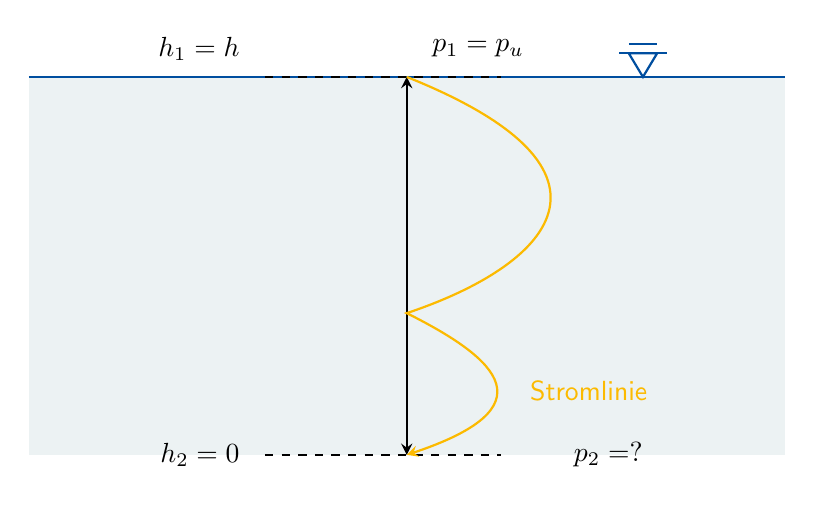
\begin{tikzpicture}[>=stealth, font=\sffamily, scale=1.2]

    % Leichte blaue Füllung zur Andeutung des Fluids (modellhaft)
    \fill[miugray!25] (-4, 0) rectangle (4, 4);

    % Wasseroberfläche
    \draw[thick, uniblau] (-4, 4) -- (4, 4);
    
    % Symbol für freie Oberfläche (Wasserspiegel)
    \draw[uniblau, thick] (2.5, 4) -- (2.65, 4.25) -- (2.35, 4.25) -- cycle;
    \draw[uniblau, thick] (2.25, 4.25) -- (2.75, 4.25);
    \draw[uniblau, thick] (2.35, 4.35) -- (2.65, 4.35);

    % Gestrichelte Linien für die Höhenniveaus
    \draw[dashed, thick] (-1.5, 4) -- (1, 4);
    \draw[dashed, thick] (-1.5, 0) -- (1, 0);

    % Pfeil für den Höhenunterschied (h)
    \draw[<->, thick] (0, 0) -- (0, 4);

    % Stromlinie (geschwungener Pfad)
    \draw[->, thick, unigelb] (0, 4) 
        .. controls (2.5, 3) and (1.5, 2) .. (0, 1.5) 
        .. controls (1,1) and (1.5,0.5) .. (0,0)
        node[pos=0.55, right=3mm] {Stromlinie};

    % Beschriftungen Oben (Niveau 1)
    \node[left=2mm] at (-1.5, 4.3) {$h_1 = h$};
    \node[right=2mm] at (0, 4.3) {$p_1 = p_u$};

    % Beschriftungen Unten (Niveau 2)
    \node[left=2mm] at (-1.5, 0) {$h_2 = 0$};
    \node[right=2mm] at (1.5, 0) {$p_2 = ?$};

\end{tikzpicture}

\end{figure}
\end{minipage}%
\hspace*{4mm}
\begin{minipage}{.5\textwidth}
\antwort{
\begin{align*}
\underbrace{p_1}_{p_u} + \frac{1}{2} \rho \underbrace{v_1^2}_{=0} + \rho g \underbrace{h_1}_{=h} &= p_2 + \frac{1}{2} \rho \underbrace{v_2^2}_{=0} + \rho g \underbrace{h_2}_{=0} \\
p_2 &= p_u + \rho g h
\end{align*}
}
\end{minipage}%


\end{frame}


\begin{frame}

\begin{minipage}{.35\textwidth}

{\color{miugray}$\blacksquare ~$} \textbf{Aufgabe 2} \par \vspace*{2mm}

\begin{figure}[h]
\centering
\resizebox{.8\textwidth}{!}{
\begin{tikzpicture}[>=stealth, scale=1.2, font=\small]

    % Parametrisierung der Koordinaten für einfache Anpassungen
    \def\rOne{1}       % Radius oben (A1)
    \def\rTwo{2.5}     % Radius unten (A2)
    \def\hTop{3.5}     % Höhe der abgeschnittenen Rohrleitung
    \def\hEntry{2}     % Höhe des Diffusoreintritts
    \def\hWater{-1}    % Höhe des Wasserspiegels
    \def\hExit{-2.5}   % Höhe des Diffusoraustritts
    \def\dimX{-3.2}    % X-Position der Bemaßungslinien

    % Wasserspiegel (Trennlinie Luft / Wasser)
    \draw (-4.5, \hWater) -- (4.5, \hWater);
    
    % Beschriftung Luft & Wasser
    \node[above right] at (-4.5, \hWater) {\large Luft};
    \node[below right] at (-4.5, \hWater) {\large Wasser};

    % Symbol für Wasseroberfläche (kleines Dreieck)
    \draw (3.2, \hWater) -- (3.4, \hWater+0.25) -- (3.0, \hWater+0.25) -- cycle;

    % Symmetrieachse (strichpunktiert)
    \draw[dotted,line width=1pt] (0, \hTop+0.5) -- (0, \hExit-0.5);

    % --- Diffusor Kontur ---
    
    % Abgeschnittenes Rohr oben (Wellenlinie)
    \draw (-\rOne, \hTop) sin (-0.5, \hTop+0.1) cos (0, \hTop) sin (0.5, \hTop-0.1) cos (\rOne, \hTop);
    
    % Vertikales Rohrstück oben
    \draw (-\rOne, \hTop) -- (-\rOne, \hEntry);
    \draw (\rOne, \hTop) -- (\rOne, \hEntry);
    
    % Eintrittsfläche A1 (Trennlinie)
    \draw (-\rOne, \hEntry) -- (\rOne, \hEntry);
    
    % Konischer Teil des Diffusors
    \draw (-\rOne, \hEntry) -- (-\rTwo, \hWater);
    \draw (\rOne, \hEntry) -- (\rTwo, \hWater);
    
    % Zylindrischer Teil unten (unter Wasser)
    \draw (-\rTwo, \hWater) -- (-\rTwo, \hExit);
    \draw (\rTwo, \hWater) -- (\rTwo, \hExit);
    
    % Austrittsfläche A2 (Bodenlinie)
    \draw (-\rTwo, \hExit) -- (\rTwo, \hExit);


    % --- Beschriftungen ---
    \node[scale=1.3] at (-0.5*\rOne, \hEntry+0.35) {$p_1$};
    \node[scale=1.3] at (-0.5*\rOne, \hEntry-0.35) {$A_1$};
    \node[scale=1.3] at (\rTwo+0.5, 0.5) {$p_0$};
    \node[scale=1.3] at (-0.5*\rTwo, \hExit+0.35) {$A_2$};

    % Pfeil für den Volumenstrom (V-Punkt)
    \draw[->,very thick] (0, \hEntry-0.5) -- (0, \hWater+0.2) node[midway, right=2pt] {$\dot{V}$};


    % --- Bemaßungen ---
    
    % Hilfslinien für Bemaßung
    \draw (-\rOne-0.2, \hEntry) -- (\dimX-0.2, \hEntry);
    \draw (-\rTwo-0.2, \hExit) -- (\dimX-0.2, \hExit);

    % Bemaßung h
    \draw[<->,very thick] (\dimX, \hEntry) -- (\dimX, \hWater) node[midway, left=2pt] {\large $h$};
    
    % Bemaßung D
    \draw[<->,very thick] (\dimX, \hWater) -- (\dimX, \hExit) node[midway, left=2pt] {\large $D$};

\end{tikzpicture}
}
\caption{Abbildung eines Austrittsdiffusors}
\end{figure}
\end{minipage}%
\hspace*{4mm}
\begin{minipage}{.65\textwidth}
\antwort{
\begin{align*}
p_1 + \rho g h_1 + \frac{1}{2}\rho v_1^2 &= p_2 + \rho g h_2 + \frac{1}{2}\rho v_2^2 \\
p_1 + \rho g h_1 + \frac{1}{2}\rho \left( \frac{\dot{V}}{A_1} \right)^2 &= p_2 + \rho g h_2 + \frac{1}{2}\rho \left( \frac{\dot{V}}{A_2} \right)^2 \\
p_1 + \rho g h_1 + \frac{1}{2}\rho \left(\frac{\dot{V}}{A_1}\right)^2 &= p_0  + \rho g D - \rho g D + \frac{1}{2}\rho \left( \frac{\dot{V}}{A_2} \right)^2 \\
p_1 + \rho g h_1 + \frac{1}{2}\rho \left( \frac{\dot{V}}{A_1} \right)^2 &= p_0  + \frac{1}{2}\rho\left(  \frac{\dot{V}}{A_2} \right)^2 \\
\end{align*}
Wir setzen $p_1$ = 0
\begin{align*}
0 + \rho g h_1 + \frac{1}{2}\rho \left( \frac{\dot{V}}{A_1} \right)^2 &= p_0  + \frac{1}{2}\rho \left( \frac{\dot{V}}{A_2} \right)^2 \\
\end{align*} 
}
\end{minipage}%


\end{frame}




\begin{frame}

\begin{minipage}{.35\textwidth}

{\color{miugray}$\blacksquare ~$} \textbf{Aufgabe 2} \par \vspace*{2mm}

\begin{figure}[h]
\centering
\resizebox{.8\textwidth}{!}{
\begin{tikzpicture}[>=stealth, scale=1.2, font=\small]

    % Parametrisierung der Koordinaten für einfache Anpassungen
    \def\rOne{1}       % Radius oben (A1)
    \def\rTwo{2.5}     % Radius unten (A2)
    \def\hTop{3.5}     % Höhe der abgeschnittenen Rohrleitung
    \def\hEntry{2}     % Höhe des Diffusoreintritts
    \def\hWater{-1}    % Höhe des Wasserspiegels
    \def\hExit{-2.5}   % Höhe des Diffusoraustritts
    \def\dimX{-3.2}    % X-Position der Bemaßungslinien

    % Wasserspiegel (Trennlinie Luft / Wasser)
    \draw (-4.5, \hWater) -- (4.5, \hWater);
    
    % Beschriftung Luft & Wasser
    \node[above right] at (-4.5, \hWater) {\large Luft};
    \node[below right] at (-4.5, \hWater) {\large Wasser};

    % Symbol für Wasseroberfläche (kleines Dreieck)
    \draw (3.2, \hWater) -- (3.4, \hWater+0.25) -- (3.0, \hWater+0.25) -- cycle;

    % Symmetrieachse (strichpunktiert)
    \draw[dotted,line width=1pt] (0, \hTop+0.5) -- (0, \hExit-0.5);

    % --- Diffusor Kontur ---
    
    % Abgeschnittenes Rohr oben (Wellenlinie)
    \draw (-\rOne, \hTop) sin (-0.5, \hTop+0.1) cos (0, \hTop) sin (0.5, \hTop-0.1) cos (\rOne, \hTop);
    
    % Vertikales Rohrstück oben
    \draw (-\rOne, \hTop) -- (-\rOne, \hEntry);
    \draw (\rOne, \hTop) -- (\rOne, \hEntry);
    
    % Eintrittsfläche A1 (Trennlinie)
    \draw (-\rOne, \hEntry) -- (\rOne, \hEntry);
    
    % Konischer Teil des Diffusors
    \draw (-\rOne, \hEntry) -- (-\rTwo, \hWater);
    \draw (\rOne, \hEntry) -- (\rTwo, \hWater);
    
    % Zylindrischer Teil unten (unter Wasser)
    \draw (-\rTwo, \hWater) -- (-\rTwo, \hExit);
    \draw (\rTwo, \hWater) -- (\rTwo, \hExit);
    
    % Austrittsfläche A2 (Bodenlinie)
    \draw (-\rTwo, \hExit) -- (\rTwo, \hExit);


    % --- Beschriftungen ---
    \node[scale=1.3] at (-0.5*\rOne, \hEntry+0.35) {$p_1$};
    \node[scale=1.3] at (-0.5*\rOne, \hEntry-0.35) {$A_1$};
    \node[scale=1.3] at (\rTwo+0.5, 0.5) {$p_0$};
    \node[scale=1.3] at (-0.5*\rTwo, \hExit+0.35) {$A_2$};

    % Pfeil für den Volumenstrom (V-Punkt)
    \draw[->,very thick] (0, \hEntry-0.5) -- (0, \hWater+0.2) node[midway, right=2pt] {$\dot{V}$};


    % --- Bemaßungen ---
    
    % Hilfslinien für Bemaßung
    \draw (-\rOne-0.2, \hEntry) -- (\dimX-0.2, \hEntry);
    \draw (-\rTwo-0.2, \hExit) -- (\dimX-0.2, \hExit);

    % Bemaßung h
    \draw[<->,very thick] (\dimX, \hEntry) -- (\dimX, \hWater) node[midway, left=2pt] {\large $h$};
    
    % Bemaßung D
    \draw[<->,very thick] (\dimX, \hWater) -- (\dimX, \hExit) node[midway, left=2pt] {\large $D$};

\end{tikzpicture}
}
\caption{Abbildung eines Austrittsdiffusors}
\end{figure}
\end{minipage}%
\hspace*{4mm}
\begin{minipage}{.65\textwidth}
\antwort{

Nach Volumenstrom umstellen und einsetzen:
\begin{align*}
\frac{1}{2}\rho \left( \frac{\dot{V}}{A_1} \right)^2 - \frac{1}{2}\rho \left( \frac{\dot{V}}{A_2} \right)^2 &= p_0 - \rho g h\\
\left( \frac{\dot{V}}{A_1} \right)^2 - \left( \frac{\dot{V}}{A_2} \right)^2 &= \frac{p_0 - \rho g h}{\frac{1}{2}\rho}\\
\dot{V} &= \sqrt{\frac{p_0 - \rho g h}{\frac{1}{2} \rho \cdot\left[ \left(\frac{1}{A_1} \right)^2 - \left(\frac{1}{A_2} \right)^2 \right] }} \\
\dot{V} &= \sqrt{\frac{100.000 - 1.000 \cdot 9,81 \cdot 2}{\frac{1}{2} \cdot 1.000 \cdot\left[ \left(\frac{1}{5~\text{m}^2} \right)^2 - \left(\frac{1}{25~\text{m}^2} \right)^2 \right] }}
\end{align*}
\begin{align*}
\dot{V} \geq 64,7 ~\text{m}^3\text{/s}
\end{align*}
}
\end{minipage}%


\end{frame}




\begin{frame}
\begin{minipage}{.5\textwidth}


{\color{miugray}$\blacksquare ~$} \textbf{Aufgabe 3} \par \vspace*{2mm}
In einer Gasleitung ($\rho_{Gas} = 1, 18 ~\text{kg/m}^3$
, $\nu_{Gas} = 15 \cdot 10^{-6} ~\text{m}^2\text{/s}$) von 0,2 km Länge und
150 mm Durchmesser strömt das Gas mit einer Geschwindigkeit von 20 m/s. Die Rauhigkeit
$k$ sei 0, 075 mm (geschweißte Stahlrohre).
Man berechne den Druckabfall $\Delta p$. Die Strömung kann als inkompressibel angenommen
werden.
\end{minipage}%
\hspace*{4mm}
\begin{minipage}{.5\textwidth}
\antwort{
Reynoldszahl:
\begin{align*}
Re &= \frac{v \cdot l}{\nu} \\
 &= \frac{20~\text{m/s} \cdot 0,15 m}{15 \cdot 10^{-6} ~\text{m$^2$/s}} \\
 &= 2 \cdot 10^5 \rightarrow ~\text{turbulent}
\end{align*}
Relative Wandrauhigkeit:
\begin{align*}
\frac{d}{k} = \frac{150}{0,075} = 2.000 \\
\frac{k}{d} = 5 \cdot 10^{-4}
\end{align*}
$\xi_{Rohr}$ aus Moody-Diagramm ablesen \RA 0,02


\begin{align*}
\Delta p &= \xi_{Rohr} \cdot \frac{l}{d} \cdot \frac{1}{2}\rho \overline{v}^2 \\
 &= 0,02 \cdot \frac{200}{0,15} \cdot \frac{1}{2} \cdot 1,18 \cdot 20^2 \\
 &= 6.293,3 ~\text{Pa}
% &= 5.82 \cdot 10^{-2}~\text{bar}
\end{align*}
}
\end{minipage}%
\end{frame}


\begin{frame}
\includegraphics[width=12cm]{F://LaTeX-Files/pngs/moody_edit.pdf}
\end{frame}


\begin{frame}
\begin{minipage}{.5\textwidth}


{\color{miugray}$\blacksquare ~$} \textbf{Aufgabe 4} \par \vspace*{2mm}
Was versteht man unter der Nusselt-Zahl und der Prandtl-Zahl? Versuchen Sie die Begriffe in anschaulichen Beispielen darzustellen
\end{minipage}%
\hspace*{4mm}
\begin{minipage}{.5\textwidth}

\antwort{ \footnotesize
Die \textbf{Nußelt-Zahl} drückt aus, um welchen Faktor die Wärmeübertragung aufgrund der Konvektion stärker ist als wenn reine Wärmeleitung wirken würde.
\begin{align*}
\text{Nu} = \frac{\text{Wärmetransport Konvektion}}{\text{Wärmetransport Leitung}} = \frac{\alpha \cdot L}{\lambda}
\end{align*}

\pp
Die \textbf{Prandtl-Zahl} kann wie folgt interpretiert werden:

\begin{itemize}
\item Eine hohe Prandtl-Zahl bedeutet, dass das Fluid eine hohe Viskosität und eine niedrige Temperaturleitfähigkeit hat.
\item Eine niedrige Prandtl-Zahl bedeutet, dass das Fluid eine niedrige Viskosität und eine hohe Temperaturleitfähigkeit hat.
\end{itemize}

\par \vspace*{-4mm}
\begin{align*}
\text{Pr} = \frac{\text{Impulstransport}}{\text{Wärmetransport}} = \frac{\nu}{\alpha}
\end{align*}

Da der Impulstransport durch das Geschwindigkeitsfeld, der Wärmetransport durch das Temperaturfeld bestimmt ist, verbindet die Prandtl-Zahl die beiden für den Wärmeübergang maßgebenden Felder. Die Prandtl-Zahl ist somit ein Maß für das Verhältnis der Dicken von Strömungsgrenzschicht zu Temperaturgrenzschicht.
}

\end{minipage}%
\end{frame}


\end{document}
